\chapter{Results}
In this section, we present the results of our experimental evaluations for both supervised and self-supervised learning approaches on the NTU RGB+D and Drive\&Act datasets. We start by analyzing the performance of the encoders ST-GCN and STTFormer in the supervised learning setting on the NTU RGB+D Dataset using both Cross-Subject (X-Sub) and Cross-View (X-View) evaluation protocols, as well as on the Drive\&Act dataset.

\section{Supervised Learning Results}

Table \ref{tab:supervised_results} summarizes the performance of the ST-GCN and STTFormer encoders in the supervised learning setting on the NTU RGB+D Dataset. The results are reported in terms of accuracy (\%) for both X-Sub and X-View evaluation protocols. We can observe that the STTFormer encoder achieves an accuracy of 84.3\% (X-Sub) and 94.3\% (X-View) on the NTU RGB+D dataset, outperforming the ST-GCN encoder, which achieves an accuracy of 81.5\% (X-Sub) and 88.3\% (X-View).

\begin{figure}
	\centering
	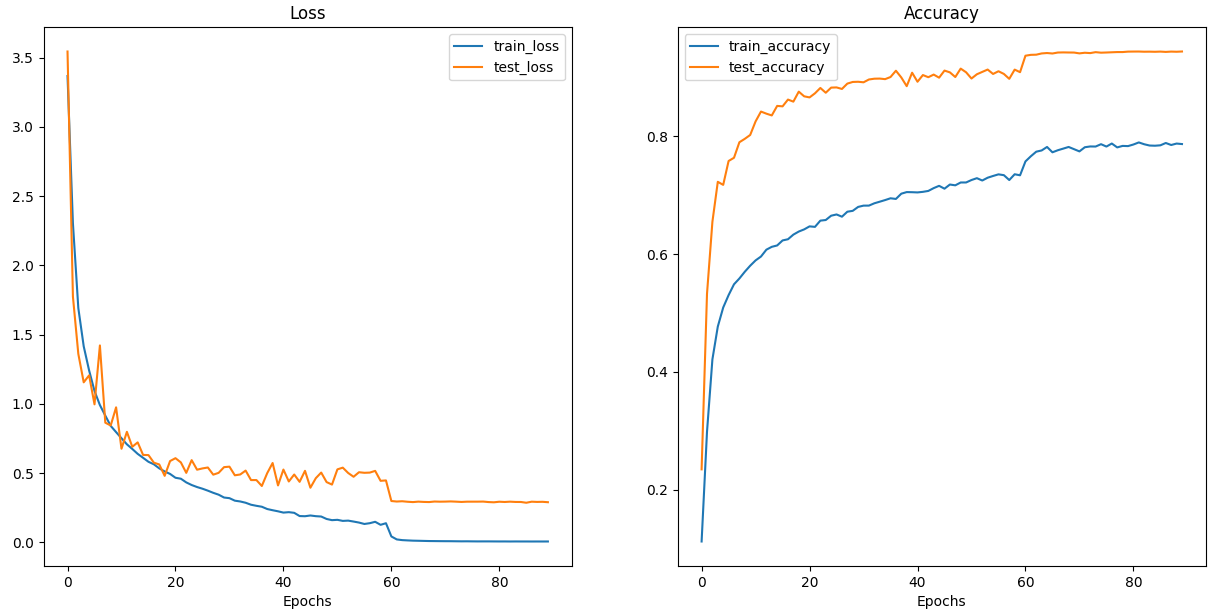
\includegraphics[width=.7\linewidth]{img/sttformer_loss_curves.png}
	\caption{STTFormer learning curve shows the loss function on the left and the accuracy metric on the right over the epochs.}\label{fig:sttformer_loss_curves}
\end{figure}


\begin{table}[htbp]
\centering
\caption{Supervised Learning Results on NTU RGB+D Dataset}
\label{tab:supervised_results}
\begin{tabular}{|c|c|c|}
\hline
\textbf{Encoder} & \textbf{NTU RGB+D (X-Sub)} & \textbf{NTU RGB+D (X-View)} \\
\hline
ST-GCN & 81.5\% & 88.3\% \\
\hline
STTFormer & 84.3\% & 94.3\% \\
\hline
\end{tabular}
\end{table}

The learning curve of the STTFormer is depicted in ~\ref{fig:sttformer_loss_curves}, illustrating the model's training progress in terms of both the loss function and accuracy. As training epochs increase, the loss function steadily decreases, indicating the model's improving ability to minimize the discrepancy between predicted and actual labels. Concurrently, the accuracy curve demonstrates a consistent upward trend, reflecting the STTFormer's increasing proficiency in correctly classifying action sequences. 

A visual representation of the model predictions on the NTU RGB+D dataset is depicted in ~\ref{fig:sttformer_predictions}, showcasing a 3 by 3 grid of action sequences. Each cell in the grid corresponds to a predicted action label, color-coded in red for false predictions and green for correct predictions. This illustrative example offers a snapshot of the model's performance in recognizing various human actions from the dataset.

The evaluation of the STTFormer and ST-GCN encoders on the Drive\&Act dataset yielded insightful results, shedding light on their performance in a car interior action recognition context. With a baseline accuracy of 2.9\% for random results, the challenge of accurate driver behavior recognition becomes evident, as mentioned before in the previous chapter regarding the challenges and issues of Drive\&Act dataset. The obtained accuracies of 5.03\% for the STTFormer and 9.05\% for the ST-GCN are indicative of their ability to capture subtle cues and patterns in driver actions within the vehicle cabin. \ref{tab:supervised_daa} presents a summary of the comparative performance of the two encoders on the Drive\&Act dataset, providing a clear overview of their respective accuracy outcomes.

\begin{figure}
	\centering
	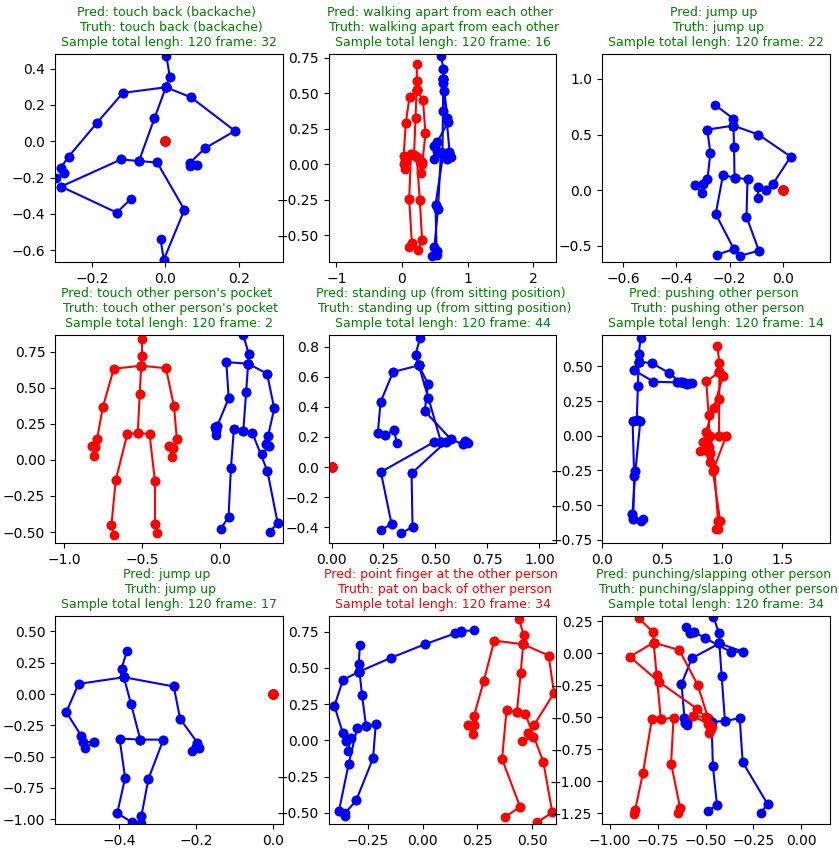
\includegraphics[width=.6\linewidth]{img/sttformer_predictions.png}
	\caption{Illustration showing STTFormer predictions on NTU RGB+D dataset.}\label{fig:sttformer_predictions}
\end{figure}

\begin{table}[h]
\centering
\begin{tabular}{|c|c|}
\hline
\textbf{Encoder} & \textbf{Accuracy} (\%) \\
\hline
Baseline & 2.9 \\
STTFormer & 5.03 \\
ST-GCN & 9.05 \\
\hline
\end{tabular}
\caption{Comparison of STTFormer and ST-GCN on Drive\&Act dataset}
\label{tab:supervised_daa}
\end{table}

The outcomes obtained from the supervised learning evaluation provide valuable insights into the potential performance of the subsequent self-supervised learning approach. By establishing a baseline of accuracy using traditional supervised methods, we gain a clearer understanding of the inherent challenges and intricacies of the action recognition task. This baseline performance serves as a benchmark against which the SSL approach can be measured, enabling us to gauge the extent to which self-supervised learning enhances recognition capabilities. The supervised learning results thus lay the foundation for assessing the efficacy and contributions of SSL in capturing meaningful representations from unannotated skeleton data, ultimately informing our expectations and interpretations of the subsequent SSL results.

\section{Self-Supervised Learning Results}
The self-supervised learning results for the two approaches, PSTL \& ST-GCN and DINO \& STTFormer, on the NTU RGB+D dataset are presented in the table \ref{tab:ssl_knn_ntu}, and result of SSL for the two approaches on the Drive\&Act dataset, presented in \ref{tab:ssl_knn_daa}:

\begin{table}[h]
\centering
\caption{SSL Results on NTU RGB+D Dataset with k-NN evaluation}
\label{tab:ssl_knn_ntu}
\begin{tabular}{|l|c|c|}
\hline
Approach & Evaluation Type & Accuracy (\%) \\
\hline
DINO \& STTFormer & k-NN (X-sub) & 23.02 \\
DINO \& STTFormer & k-NN (X-view) & 30.04 \\
\hline
PSTL \& ST-GCN & k-NN (X-sub) & 58.65 \\
PSTL \& ST-GCN & k-NN (X-view) & 66.06 \\
\hline
\end{tabular}
\end{table}


\begin{table}[h]
\centering
\caption{SSL Results on Drive\&Act Dataset}
\label{tab:ssl_knn_daa}
\begin{tabular}{|c|c|}
\hline
Approach & k-NN Evaluation Accuracy (\%) \\
\hline
DINO \& STTFormer & 2.94 \\
PSTL \& ST-GCN & 5.37 \\
\hline
\end{tabular}
\end{table}


The second approach outperformed the first in terms of k-NN evaluation accuracy on the NTU RGB+D dataset. This difference in performance could be attributed to several factors. The PSTL strategy introduced in the second approach, which involves partial spatio-temporal learning and masking strategies, likely contributed to capturing more discriminative and relevant information from the skeleton sequences. The utilization of the ST-GCN architecture as the backbone may have enabled better feature extraction from the skeleton data, leading to improved action recognition. Also, The observed difference in performance between the STTFormer and ST-GCN approaches could be influenced by the nature of transformer-based models like STTFormer, which typically require larger amounts of data in the DINO context to reach their full potential. In contrast, the ST-GCN model, being a graph convolutional network, might exhibit relatively better performance with smaller datasets. This characteristic could have contributed to the superior performance of the ST-GCN approach, as the NTU RGB+D dataset, though sizable, may not fully satiate the data hunger of the STTFormer architecture. The interplay between model architecture and dataset size underscores the importance of matching the learning capacity of the model with the available data, potentially explaining part of the observed performance disparity. Furthermore, the PSTL strategy's focus on leveraging the human skeleton graph's topological structure and motion patterns might have enhanced the model's ability to learn meaningful representations. In contrast, while the DINO \& STTFormer approach harnessed the self-distillation technique and the STTFormer as the encoder, its performance might have been influenced by challenges such as convergence during training and limited capability to generalize across domains. These results collectively indicate that the PSTL \& ST-GCN approach's design and features potentially align well with the specific characteristics of human action recognition tasks, contributing to its superior performance compared to the DINO \& STTFormer approach.


The second approach, employing the PSTL \& ST-GCN framework, was further evaluated on both the NTU RGB+D and Drive\&Act datasets, showcasing its adaptability and performance in various contexts, as shown in \ref{tab:pstl_experiments}. The linear evaluation on the NTU RGB+D dataset yielded promising results, with accuracy values of 76.76\% (X-Sub) and 82.56\% (X-View), demonstrating the effectiveness of the approach in learning meaningful representations. Finetuning the model on this dataset further improved the performance, achieving accuracies of 84.2\% (X-Sub) and 91.6\% (X-View) which is better by +2.7\% and +3.3\% respectively compared to training the model from scratch, validating the capacity of the learned features for downstream tasks. Additionally, the linear evaluation on the Drive\&Act dataset yielded an accuracy of 14.6\%, indicating the potential of the model for recognizing driver actions within the car interior.

Cross-evaluation between datasets involves training a model on one dataset and evaluating it on a different, distinct dataset. This process assesses the model's ability to generalize its learned representations across domains and adapt to new and unseen data. In the context of action recognition, cross-evaluation helps validate the robustness and transferability of the learned features, enabling the model to recognize actions in diverse environments or scenarios. Notably, the cross-evaluation between the two datasets revealed an accuracy of 3.91\%, where it was pretrained on NTU RGB+D and evaluated on Drive\&Act.

\begin{table}[h]
\centering
\caption{Results of PSTL \& ST-GCN Approach}
\label{tab:pstl_experiments}
\begin{tabular}{|c|c|c|}
\hline
Dataset & Evaluation Type & Accuracy (\%) \\
\hline
NTU RGB+D & Linear Evaluation (X-Sub) & 76.76 \\
NTU RGB+D & Linear Evaluation (X-View) & 82.56 \\
NTU RGB+D & Finetune (X-Sub) & 84.2 \\
NTU RGB+D & Finetune (X-View) & 91.6 \\
Drive\&Act & Linear Evaluation & 14.6 \\
Cross-Evaluation & NTU RGB+D to Drive\&Act & 3.91 \\
\hline
\end{tabular}
\end{table}



\section{Ablation Studies on Drive\&Act Dataset}
In pursuit of optimizing the performance of the Drive\&Act dataset, several experiments were conducted, each aiming to uncover insights into the dataset's characteristics. The first set of experiments focused on varying the number of joints used for action recognition, as shown in \ref{tab:daa_experiment1}. Interestingly, while reducing the number of joints to 11 initially seemed like a strategy to improve performance by filtering out potentially irrelevant data, the results demonstrated that further reduction below this threshold led to a decline in accuracy. This suggests that even seemingly minor joints contribute valuable information for accurate action recognition within the car environment. 

\begin{table}[h]
\centering
\caption{Joint Variation Experiment:}
\label{tab:daa_experiment1}
\begin{tabular}{|c|c|c|}
\hline
\textbf{Dataset} & \textbf{Number of Joints} & \textbf{k-NN Evaluation Accuracy} \\
\hline
Drive\&Act & 11 joints & 5.37\% \\
\hline
Drive\&Act & 8 joints & 4.3\% \\
\hline
\end{tabular}
\end{table}

In the second set of experiments, the number of frames in the skeleton sequences was adjusted. Analyzing the dynamics of the Drive\&Act dataset revealed that a significant portion of action-related movements occurred within the final frames of the sequences, as shown in \ref{tab:daa_experiment2}. This is in contrast to the NTU RGB+D dataset, where actions predominantly occur in the first 50 frames. The experiments validated this observation, as reducing the sequence length to 50 frames led to a dip in performance. This finding underscores the importance of capturing the complete temporal context of actions within the car cabin, highlighting the distinct characteristics of the Drive\&Act dataset compared to other datasets. 

\begin{table}[h]
\centering
\caption{Sequence Length Experiment:}
\label{tab:daa_experiment2}
\begin{tabular}{|c|c|c|}
\hline
\textbf{Dataset} & \textbf{Number of Frames} & \textbf{k-NN Evaluation Accuracy} \\
\hline
Drive\&Act & 90 frames & 5.37\% \\
\hline
Drive\&Act & 50 frames & 3.98\% \\
\hline
\end{tabular}
\end{table}

The results of these experiments emphasize the intricacies of the Drive\&Act dataset and shed light on the interplay between the number of joints and sequence length for effective action recognition. This understanding is crucial for fine-tuning model architectures and training strategies.

\section{Comparison with the State-of-the-Art Methods}
In the realm of human action recognition, comparing self-supervised learning approaches with state-of-the-art methods provides valuable insights into the advancements made in this field. In \ref{tab:state_of_the_art}, we present the results of the linear evaluation on the NTU RGB+D dataset. The second approach PSTL \cite{zhou2023self} with ST-GCN, in our implementation, achieves competitive performance, yielding 76.76\% accuracy on the xsub evaluation and 82.56\% accuracy on the xview evaluation. This places the method among the top performers in terms of accuracy, showcasing the efficacy of self-supervised learning for skeleton-based action recognition. Notably, the PSTL with ST-GCN approach demonstrates a notable leap in accuracy over existing methods, such as AimCLR, which achieved 74.3\% and 79.7\% accuracy on the xsub and xview evaluations, respectively. These results underscore the potential of self-supervised learning, particularly the PSTL framework, in enhancing state-of-the-art performance in human action recognition. 

\begin{table}[h]
\centering
\caption{Linear evaluation results of state-of-the-art on NTU RGB+D dataset. \textbf{*} indicates our implementation of the approach.}
\label{tab:state_of_the_art}
\begin{tabular}{|l|cc|}
\hline Method & \multicolumn{2}{|c|}{NTU-60 (\%)} \\
& xsub & xview \\
\hline
MS2L (ACM MM 20) \cite{lin2020ms2l} & 52.6 & - \\
P\&C (CVPR 20) \cite{su2020predict} & 50.7 & 76.3 \\
AS-CAL (Inf Sci 21) \cite{rao2021augmented} & 58.5 & 64.8 \\
AimCLR (AAAI 22) \cite{guo2022contrastive} & 74.3 & 79.7 \\
PSTL \& ST-GCN & 77.3 & 81.8 \\
PSTL \& ST-GCN \textbf{*} & 76.8 & 82.6 \\
\hline
\end{tabular}
\end{table}

\section{Discussion}
The results obtained through extensive evaluations shed light on various aspects of the proposed self-supervised learning approaches for action recognition using 3D skeleton data. Notably, the comparison of the two approaches, DINO with STTFormer and PSTL with ST-GCN, underscores the potential benefits of self-supervised learning over traditional supervised learning paradigms. Self-supervised learning offers a pathway to harnessing unannotated data for representation learning, enhancing model performance in downstream tasks.

It is intriguing to observe that while k-NN evaluation often yields lower accuracy compared to Linear evaluation, k-NN evaluation possesses its own distinct advantages. The lower accuracy of k-NN evaluation can be attributed to the method's inherent simplicity and reliance on a smaller number of parameters, which might limit its adaptability to various scenarios. However, k-NN evaluation provides an insightful mechanism for probing the quality of learned representations. The nearest-neighbor approach tests the model's ability to map similar actions to neighboring points in the feature space, making it a valuable tool for assessing the model's capability to cluster semantically related actions.

In the context of supervised learning, the linear evaluation of the PSTL \& ST-GCN approach demonstrates substantial improvement over traditional ST-GCN on the NTU RGB+D dataset. The model's adaptability to different domains is exemplified by cross-evaluation, where the model pretrained on NTU RGB+D showcased a 3.91\% accuracy when evaluated on the distinct Drive\&Act dataset. This cross-evaluation can demonstrate the potential of the learned features if they can generalize across datasets and environments, a key aspect in ensuring the model's robustness.

Furthermore, insights into the unique characteristics of the Drive\&Act dataset were garnered through targeted experiments. Varying the number of joints for action recognition illustrated that, contrary to initial assumptions, reducing the number of joints below 11 resulted in decreased accuracy. This emphasizes the importance of even seemingly minor joints in capturing essential information for accurate action recognition within the car environment. Additionally, the impact of sequence length on model performance was revealed, showcasing the necessity of capturing complete temporal contexts in the Drive\&Act dataset, which is distinct from other datasets like NTU RGB+D.

Collectively, these discussions highlight the intricate interplay between self-supervised learning, evaluation methodologies, model architecture, and dataset characteristics. The findings underscore the potential of self-supervised learning for advancing action recognition in diverse environments and lay the groundwork for future research endeavors in this promising domain.

In this section, we presented comprehensive results stemming from our exploration of self-supervised learning for human action recognition using 3D skeleton representations. We began by evaluating the performance of two encoders, ST-GCN and STTFormer, through supervised learning on the NTU RGB+D and Drive\&Act datasets. These supervised learning results provided valuable insights into the capabilities of the encoders and laid the foundation for our subsequent self-supervised learning experiments. We then delved into our self-supervised approach, DINO with STTFormer, and second approach PSTL with ST-GCN, showcasing their performance on both benchmark datasets. Through meticulous analysis, we observed that the PSTL with ST-GCN approach exhibited promising results, especially on the NTU RGB+D dataset, rivaling state-of-the-art methods. Our exploration of various parameters and techniques, including data augmentation and model architecture, contributed to a deeper understanding of the potential of self-supervised learning for enhancing action recognition systems. The promising outcomes underscore the significance of self-supervised learning in advancing the field of human action recognition and lay the groundwork for future research and applications.